\appendix
\chapter*{Appendix}
\addcontentsline{toc}{chapter}{Appendix}

\begin{figure}[h]
    \lstinputlisting{../assets/mermaid-example.txt}
    \caption{Example Mermaid.js code for the graph in \autoref{fig:mermaid-example-graph}}
    \label{lst:mermaid-example-code}
\end{figure}

\hspace{3cm}

\begin{figure}[h]
    \centering
    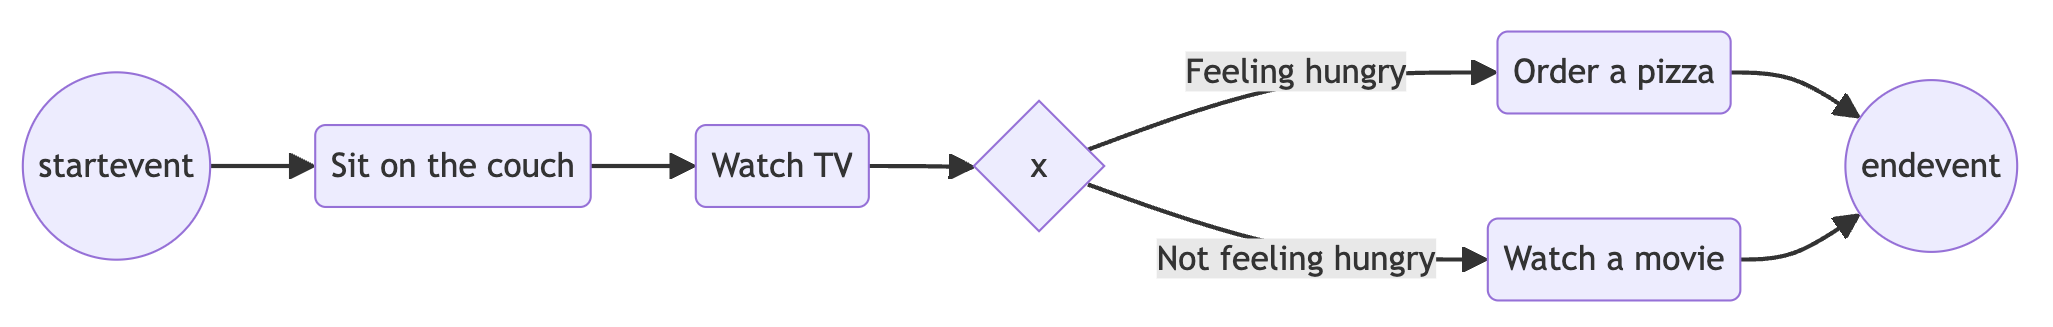
\includegraphics[width=\textwidth,keepaspectratio]{../assets/images/Mermaid Graph Example.png}
    \caption{Example Mermaid.js graph for code in \autoref{lst:mermaid-example-code}}
    \label{fig:mermaid-example-graph}
\end{figure}

\begin{figure}[h]
    \centering
    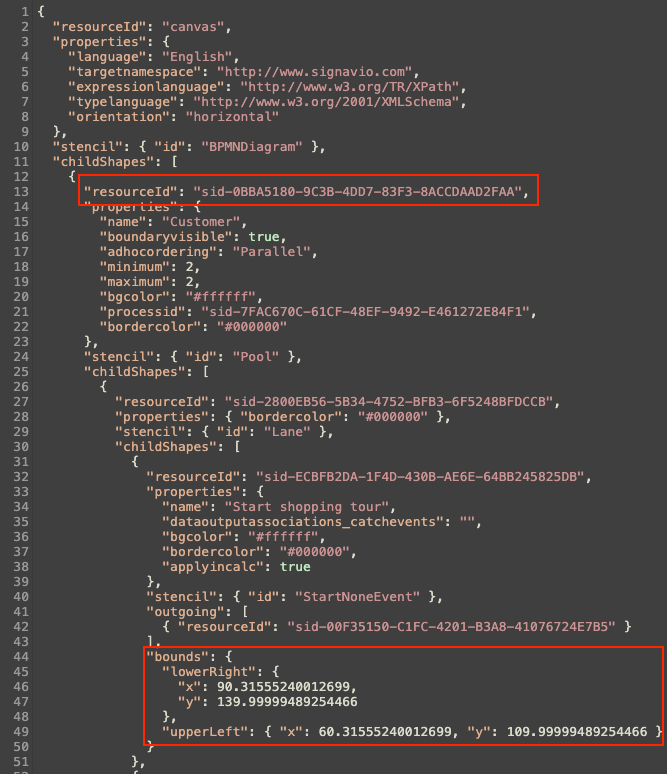
\includegraphics[width=\textwidth,height=\textheight,keepaspectratio]{../assets/images/Supermarket Shopping Signavio BPMN JSON Code Example.png}
    \caption{Extract of \gls{signavio}-compliant \acs{bpmn} 2.0 \acs{json} Code}
    \label{fig:code-example}

    \medskip
    \small
    The first 50 lines of the \acs{json} code are shown. A contained \acs{id} and the included coordinates of an element are highlighted. In the following code (not shown), more \acs{bpmn} 2.0 elements follow as part of the ``childShapes'' array in line 25 as well as an array of associations.
\end{figure}


\begin{figure}[h]
    \lstinputlisting[basicstyle=\scriptsize]{../assets/mermaid-code-prompt.txt}
    \caption{Prompt for generating a Mermaid.js graph}
    \label{lst:mermaid-prompt}
\end{figure}

\begin{figure}[h]
    \lstinputlisting[basicstyle=\scriptsize]{../assets/process-description-transcriber-1.txt}
    \caption{Example process description}
    \label{lst:mermaid-test-input}

    \medskip
    \small
    Used as input to evaluate the Mermaid.js approach (see \autoref{sec:mermaid-approach}). See the generated output in \autoref{fig:mermaid-test-output}.
\end{figure}


\begin{landscape}
    \begin{figure}[h]
        \centering
        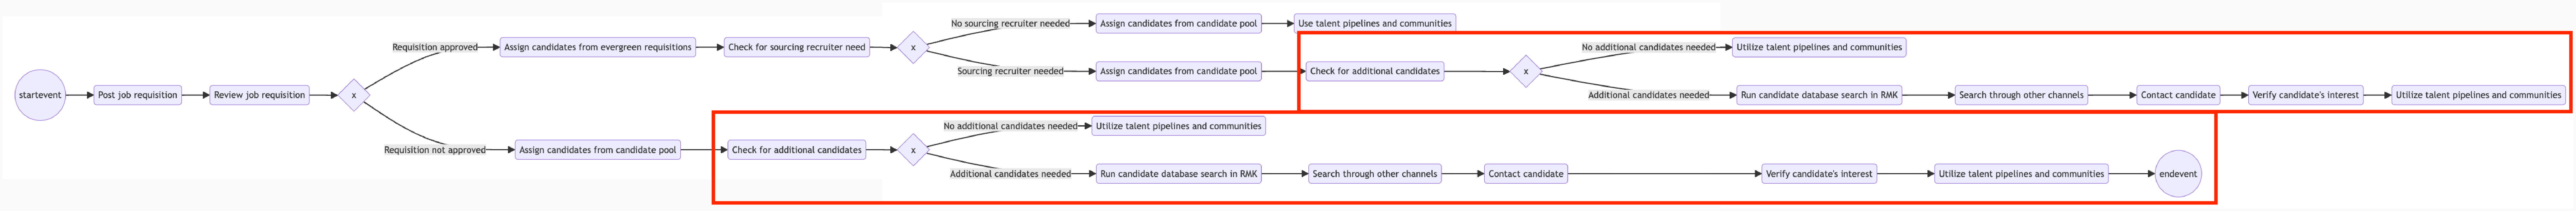
\includegraphics[width=\textheight,keepaspectratio]{../assets/images/Mermaid Test Output.png}
        \caption{Generated Mermaid.js graph}
        \label{fig:mermaid-test-output}

        \medskip
        \small
        Output of the Mermaid.js approach (see \autoref{sec:mermaid-approach}) for the process description in \autoref{lst:mermaid-test-input}. Two duplicate sequence flows are highlighted.
    \end{figure}
\end{landscape}

\begin{figure}[h]
    \lstinputlisting[basicstyle=\scriptsize]{../assets/traces-prompt.txt}
    \caption{Prompt for extracting a unique set of \glspl{trace} from a process description}
    \label{lst:traces-prompt}
\end{figure}

\begin{figure}[h]
    \lstinputlisting[basicstyle=\scriptsize]{../assets/traces-example.txt}
    \caption{Example of a unique set of \glspl{trace}.}
    \label{lst:traces-example}
\end{figure}

\begin{figure}[h]
    \lstinputlisting[basicstyle=\scriptsize]{../assets/traces-test-input.txt}
    \caption{Tested input process description for diagram in \autoref{fig:traces-test-output}.}
    \label{lst:traces-test-input}
\end{figure}

\begin{figure}[h]
    \lstinputlisting[basicstyle=\scriptsize]{../assets/traces-test-traces.txt}
    \caption{Generated set of traces (artificial \gls{event log}) for the input process description in \autoref{lst:traces-test-input}.}
    \label{lst:traces-test-traces}
\end{figure}

\begin{figure}[h]
    \lstinputlisting[basicstyle=\scriptsize]{../assets/hard-process-description.txt}
    \caption{Example of a more complex process description}
    \label{lst:hard-description}
\end{figure}